\documentclass[10pt]{beamer}

\usetheme{sidebar}
\usepackage[italian]{babel}
\usepackage[utf8x]{inputenc}
\usepackage {eurosym}
\setbeamercovered{transparent}

%
% The following info should normally be given in you main file:
%
\setbeamertemplate{footline}{
\hfill \begin{center}
 \textbf{Pagina \insertframenumber, di \inserttotalframenumber }
\end{center}

}
\title{Revisione di qualifica}
\author{Team QuiXoft}
\date{12 Marzo 2009}


\begin{document}
\transduration{1}

\frame{
	\transsplitverticalin
	\titlepage 
\begin{center}
 
\includegraphics[scale=0.20]{logo.png}
\end{center}
}
\part{Definizione di prodotto}

\frame{
	\transsplitverticalin
	\partpage }

\section{Definizione di prodotto}
\subsection{Model}
\frame{
	\frametitle{Definizione di prodotto}
  \framesubtitle{Model}
   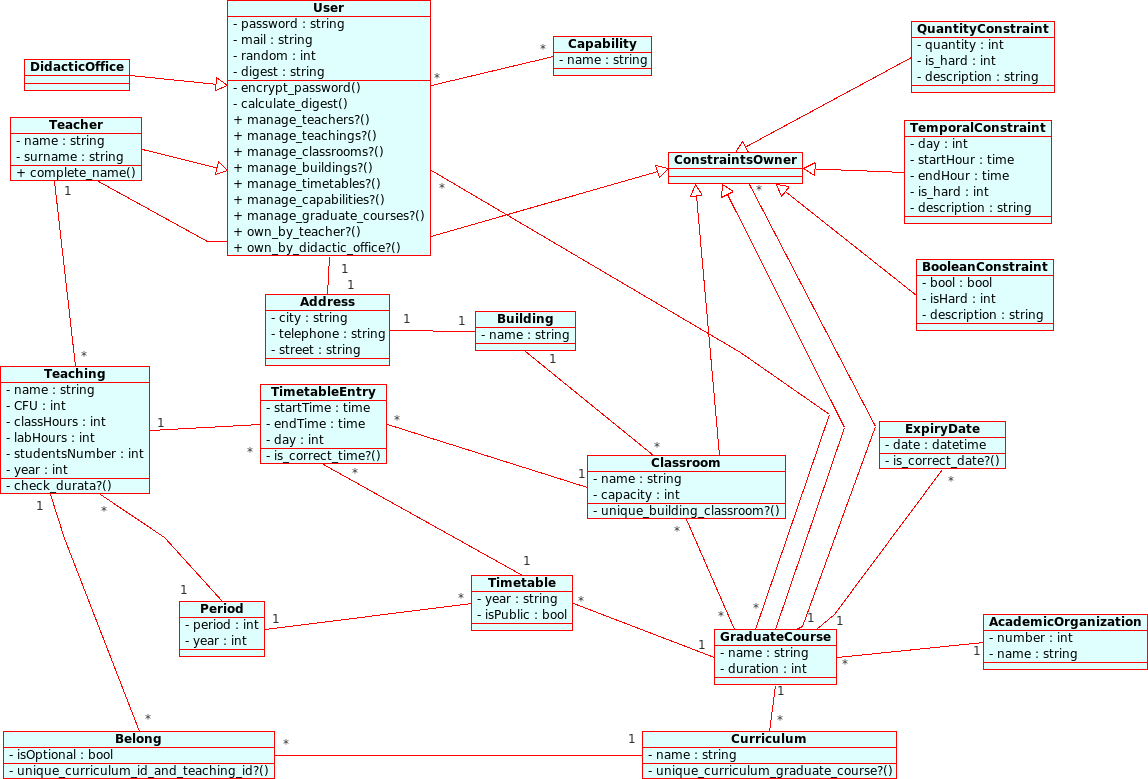
\includegraphics[scale=0.20]{images/model_diagram.png}
  \transsplitverticalin
	 }
\frame{
	\frametitle{Definizione di prodotto}
  \framesubtitle{Model}
  \transsplitverticalin
	 }

\subsection{Controller}
\frame{
	\frametitle{Definizione di prodotto}
  \framesubtitle{Controller}
  \transsplitverticalin
	 }
\frame{
	\frametitle{Definizione di prodotto}
  \framesubtitle{Controller}
  \transsplitverticalin
	 }

\subsection{View}
\frame{
	\frametitle{Definizione di prodotto}
  \framesubtitle{View}
  \transsplitverticalin
	 }
\subsection{Helper}
\frame{
	\frametitle{Definizione di prodotto}
  \framesubtitle{Helper}
  \transsplitverticalin
	 }

\subsection{MiddleMan}
\frame{
	\frametitle{Definizione di prodotto}
  \framesubtitle{War architecture}
  \transsplitverticalin
WAR-Based Mode
\begin{itemize}
\item Web ARchive (WAR)
\item standard packaging format per applicazioni su Java EE servers
\item Warbler plugin per comprimere l'applicazione Ruby-on-Rails
\end{itemize}
	 }
\frame{
	\frametitle{Definizione di prodotto}
  \framesubtitle{War architecture}
  \transsplitverticalin
\begin{center}
 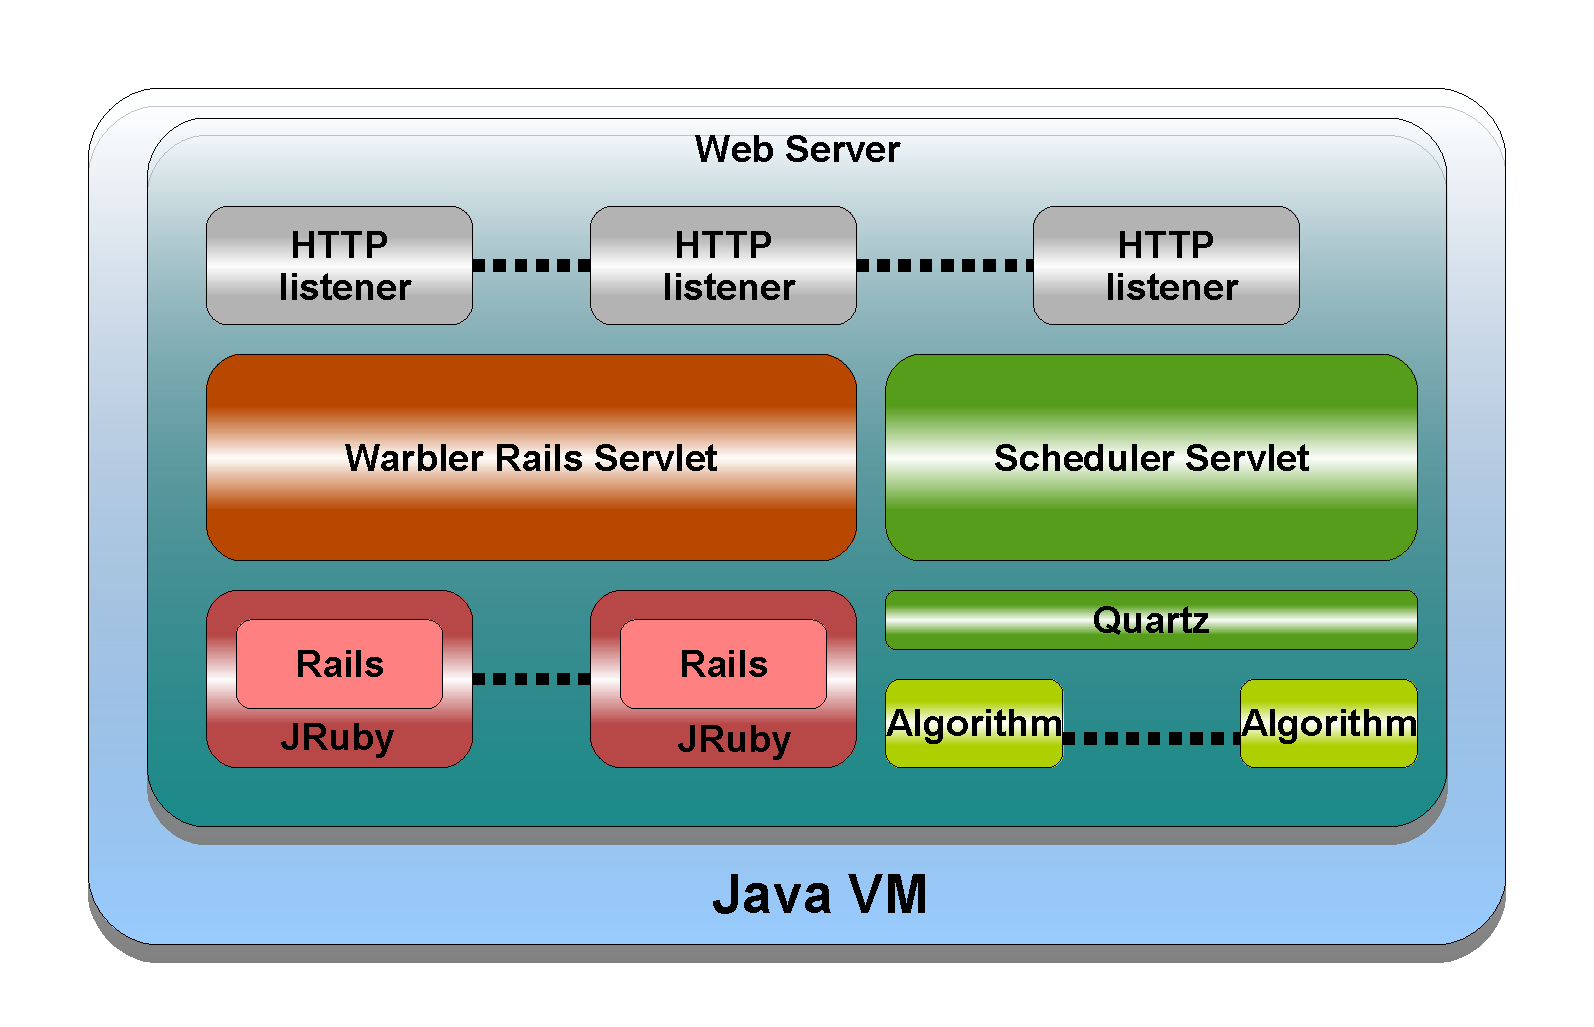
\includegraphics[scale=0.35]{images/sigeol_war_arch.pdf}
 % .: 8x8 pixel, 0dpi, infxinf cm, bb=
\end{center}
	 }
\frame{
	\frametitle{Definizione di prodotto}
  \framesubtitle{Quartz scheduler}
  \transsplitverticalin
From BackgroundRB to Quartz scheduler
\\Perchè Quartz:
\begin{itemize}
 \item semplicità di configurazione
 \item persistenza dei trigger e dei job, che possono essere salvati su database in modo trasparente
 \item clusterizzazione, quartz è stato progettato per essere cluterizzato
 \item estensibilità delle funzioni tramite plugin
 \item possibilità di monitorare tutti gli aspetti della schedulazione e di tenere traccia dell'esito dei ogni job
\end{itemize} 
}

\frame{
	\frametitle{Definizione di prodotto}
  \framesubtitle{Sequence diagram}
  \transsplitverticalin
\begin{center}
 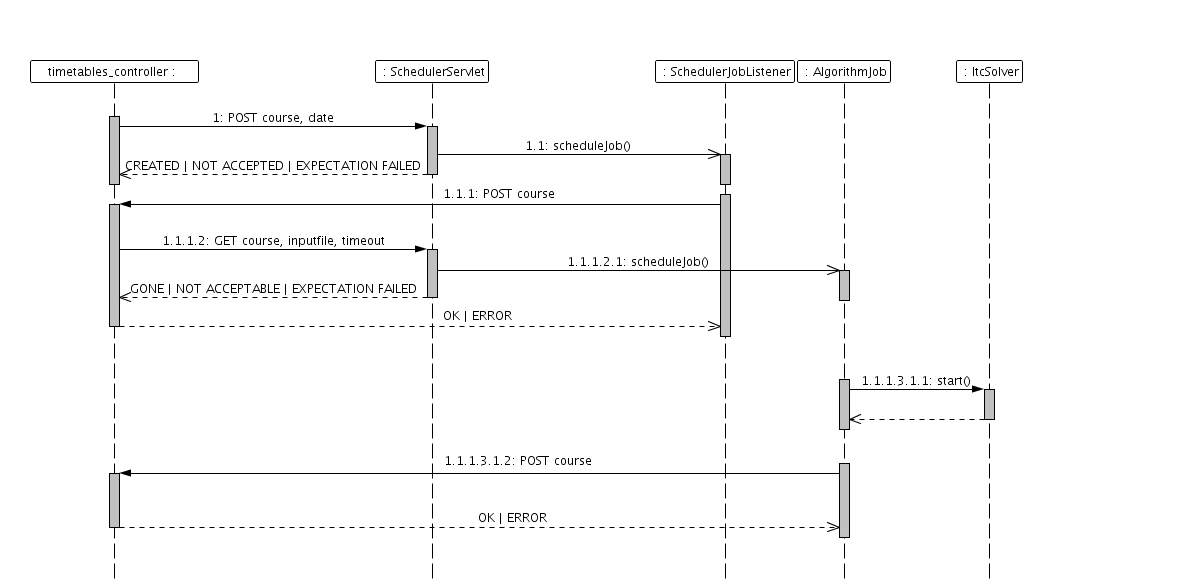
\includegraphics[scale=0.3]{images/MiddleMan_sequence_diagram.png}
 % .: 8x8 pixel, 0dpi, infxinf cm, bb=
\end{center}

	 }
\subsection{Algorithm}
\frame{
	\frametitle{Definizione di prodotto}
  \framesubtitle{Algorithm}
    \large{\textbf{Scelta dell'algoritmo}} \bigskip
    \begin{itemize}
     \item Riutilizzo di un algoritmo già esistente
     \item International Timetabling Competition 2007 (terminata in agosto 2008)
     \item Algoritmo di Tomáš Müller, vantaggi:
     	\begin{itemize}
	\item free sotto licenza LGPL
 	\item scritto in Java, interfacciamento tramite JRuby
	\item possibilità di impostare un timeout
	\item modulare e (secondo l'autore) facile da estendere
	\item ampia e chiara documentazione
	\item vincitore dell'ITC 2007
	\end{itemize}

    \end{itemize}
}
\frame{
	\frametitle{Definizione di prodotto}
  \framesubtitle{Algorithm}
  \large{\textbf{Specializzazione}} \bigskip
    \begin{itemize}
     \item Mancanza di due funzionalità importanti:
     \begin{itemize}
	\item preferenze dei docenti
	\item segnalazione delle preferenze non rispettate
     \end{itemize}
     \item studio dell'algoritmo
     \item aggiunta delle funzionalità mancanti
     \item test

    \end{itemize}
}

\part{Piano di qualifica}
\frame{
	\transsplitverticalin
	\partpage }
\subsection{Aggiornamento piano di qualifica}
\frame{
  \frametitle{Piano di qualifica}
  \framesubtitle{Aggiornamento piano di qualifica}
\begin{itemize}
 \item Tickets e consultazione ore di lavoro \bigskip
 \item Validazione automatica delle pagine web \bigskip
 \item Mocks objects \bigskip
 \item Metriche sulla copertura dei test sul codice \bigskip
\end{itemize}
}
\part{Piano di progetto}
\frame{
	\transsplitverticalin
	\partpage }
\subsection{Confronto delle ore di Analisi}
\frame{
  \frametitle{Piano di progetto}
  \framesubtitle{Confronto delle ore di Analisi}
	\transsplitverticalin
	\begin{center}
 Costo stimato: 5218\euro; costo effettivo: 5196\euro.
\end{center}
	 }
\subsection{Confronto delle ore di Progettazione e Realizzazione}
\frame{
	\frametitle{Piano di progetto}
	\framesubtitle{Confronto delle ore di Progettazione e Realizzazione}
	\transsplitverticalin
	\begin{center}
 Costo stimato totale 13793\euro.
\end{center}
	 }
\end{document}